\subsubsection{18.11.14}

\begin{enumerate}
	\item The time of beginning and ending of the congregation:
	16:00 - 1:00
	\item Purposes of the congregation:
	\begin{enumerate}
	  \item To train on control of robot.
	  
    \end{enumerate}
    
	\item Work, that has been done:
	\begin{enumerate}
	  \item The first tests of the robot showed the failure of the idea installation inside the tube plastic bottle. It reduced internal diameter of the pipe and when there is several balls in the bucket they prevent with each other to pass through the pipe. It was decided to remove the bottle. It solved this problem but now the length of tube too small for throwing of balls to baskets.
      
      \item It was turned out that STB can't turn the bucket when it filled with balls. For correction of this problem at the top part of bucket it was installed fishing cargo mass 100g.
      
     % \begin{figure}[H]
     % 	\begin{minipage}[h]{0.2\linewidth}
     % 		\center  
     % 	\end{minipage}
     % 	\begin{minipage}[h]{0.6\linewidth}
     % 		\center{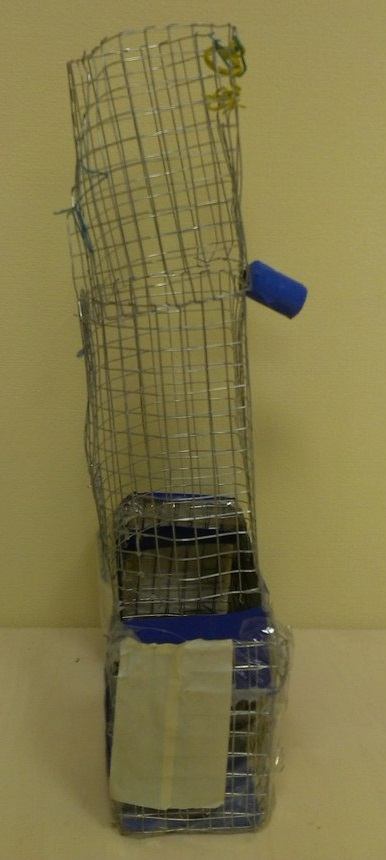
\includegraphics[scale=0.3]{days/18.11.14/images/01}}
     % 		\caption{Противовес на ковше}
     % 	\end{minipage}
     % \end{figure}
      
      \item Also it was turned out that two motors can't extract the lift. Due to this fuses are heated and unlock the chain and operator loses the control of lift. For reducing of load to motors it was decided install transmission with the ratio 1:2.
      
     % \begin{figure}[H]
     % 	\begin{minipage}[h]{0.2\linewidth}
     % 		\center  
     % 	\end{minipage}
     % 	\begin{minipage}[h]{0.6\linewidth}
     % 		\center{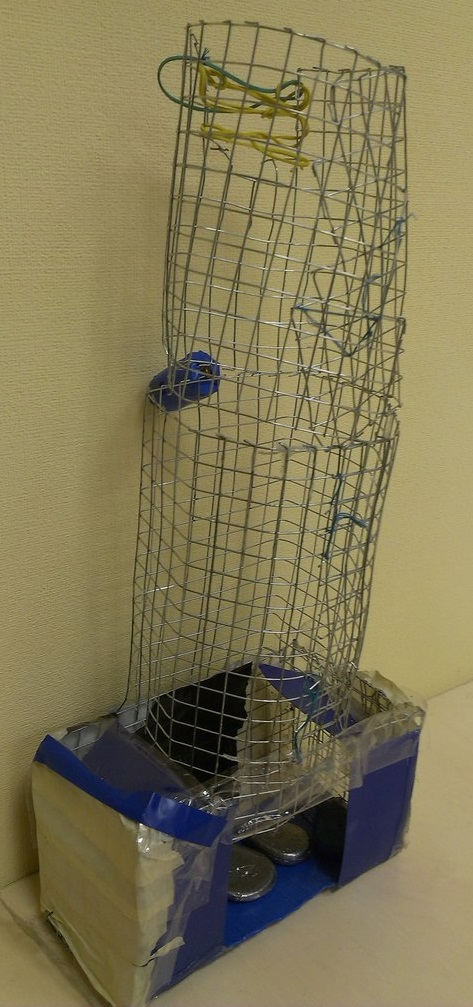
\includegraphics[scale=0.3]{days/18.11.14/images/02}}
     % 		\caption{Механизм лебедки с передаточным отношением 1:2}
     % 	\end{minipage}
     % \end{figure}
      
      \item After installation of transmission motors copes with extracting the lift but sometimes the lift was jammed. It happens due to the  clamping of the belt between top crossbar of the bottom slat and bottom crossbar of the second slat. To avoid this it was decided to install limiters that will not allow to bottom crossbar of the second slat raise too highly.
          
    \end{enumerate}
    
	\item Results:
	\begin{enumerate}
	  \item Plastic bottles was removed from the bucket. 
	  
      \item At the motors which extracts the lift it was installed transmission with the ratio 1:2.
      
      \item For normaly working of STB it was installed the cargo.
    \end{enumerate}
    
	\item Tasks for the next congregations:
	\begin{enumerate}
	  \item Install the limiters of moving of crossbar at the lift.
	  
	  \item To extend the tube of bucket for throwing of balls to baskets.
	  
	  \item To train on the control of robot.

    \end{enumerate}     
\end{enumerate}
\fillpage